	\documentclass[12pt,a4paper,oneside]{article}
	\usepackage[utf8x]{inputenc}
	\usepackage{ucs}
	\usepackage{amsmath}
	\usepackage{amsfonts}
	\usepackage{amssymb}
	\usepackage{times} % for Times New Roman Font
	\usepackage[left=1.00in, right=1.00in, top=1.00in, bottom=1.00in]{geometry}
	\usepackage{graphicx}
	
	\usepackage{algorithm} % package for writing algorithms
	\usepackage{algorithmic}
	%\usepackage{algpseudocode} % package for writing pseudocodes
	
	% packages for working schedule
	\usepackage{tikz}
	\usepackage{pgfgantt}
	
	% Package for eps graphics files
	\usepackage{epstopdf}
	
	\numberwithin{equation}{section}
	\numberwithin{algorithm}{section}
	
	\setlength{\parskip}{1.0ex plus 0.5ex minus 0.5ex}
	\setlength{\parindent}{0em}
	\setcounter{secnumdepth}{4} % Subsection level count
	
	%\usepackage{natbib} % package for bibliography style
	\renewcommand{\refname}{Bibliography}
	
	\begin{document}
	
	%\title{Off-line Nepali Handwriting Recognition Using MLP and RBF Neural Networks}
	%
	%\author{\textit{Ashok Kumar Pant}\\ \small{ashokpant87@gmail.com}\\\small{977-9849192343}}
	%\maketitle
	% First Page
\pagestyle{empty}
\begin{figure}[tp] % inserting CDCSIT Logo
\centering

\includegraphics[width=90pt]{figures/logo}
\end{figure}


\begin{center}
 {\Large \textbf{{Off-line Nepali Handwriting Recognition Using MLP and RBF Neural Networks }}}\par		%Title of dissertation
 
 
 {\large \textbf{{A Dissertation Proposal}\\}}
  
\begin{figure}[hbtp]
 \centering
 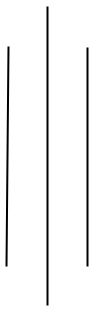
\includegraphics[width=45pt,height=100pt]{figures/vlines}
\end{figure}
  
  {\Large \textbf{{Submitted By}\\}}	% Dissertation Submitted by
  {\Large Ashok Kumar Pant\\\large Roll No. 12\\ \large Date: 10 Apr 2012}\par
           
\begin{figure}[hbtp]
 \centering
 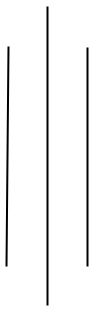
\includegraphics[width=45pt,height=100pt]{figures/vlines}
\end{figure}
  
{\Large \textbf{{Submitted To}\\}}	% Dissertation Submitted to
{\large Central Department of Computer Science and Information Technology\\
					Kirtipur, Kathmandu, Nepal }\par
					
{\Large\vspace*{5mm} \textbf {Under the Supervision of}\\
			\vspace*{3mm}\large Prof. Dr. Shashidhar Ram Joshi }\par % Supervisor
{\Large\vspace*{2mm} and \par\vspace*{2mm} \textbf{Co-Supervision of}\\
			\vspace*{3mm}\large Dr. Sanjeeb Prasad Panday}\par % Supervisor
\end{center}
	\pagestyle{plain}
	\pagenumbering{arabic}
	
	\section{Introduction} \label{introduction}
	Off-line handwriting recognition is the task of determining what characters or words are present in a digital image of handwritten text. The problem of handwriting recognition can be viewed as a classification problem where we need to identify the most suitable character the given figure matches to. It is a sub-field of Optical Character Recognition (OCR), whose domain can be machine-print or handwriting but is more commonly machine-print. The recognition of Nepali Handwritten text present unique challenges and benefits, as it belongs to devnagari script then the recognition of text in other script like Roman, Arabic, chinese, etc.
	
	A recognition system can either be on-line or off-line. In on-line recognition system the real time temporal information about the character being written is available such as the stroke order, pen up and pen down time, sequence of points traced, etc. Generally on-line recognition is preformed in fixed writing bench with some digital pen or plotter.  Operating in off-line mode gives as input the complete picture of character that we need to recognize. We don't have any temporal information about the text written. The input to off-line recognition system is the image captured with digital camera or scanned with some digital scanner. The on-line problem is somewhat easier than off-line since there is more information available.
	
	Artificial neural network is non-linear,parallel, distributed, highly connected network having capability of adaptivity, self-organization, fault tolerance, evidential response and VLSI (Very Large Scale Integration) implementation which closely resembles with physical nervous system. Physical nervous system is highly parallel, distributed information processing system having high degree of connectivity with capability of self learning. Virtual intelligence can be mimicked with the help of Artificial Neural Network (ANN). Artificial neural network algorithms can be used to simulate the real, complex biological nervous system to solve the real world problems with good performance (e.g. as measured by good predictive ability, low generalization error), or performance mimicking human error patterns, as the information processing is done in the brain. The main idea behind using ANN as recognition system is its close resemblance with physiological nervous system. Application areas of ANNs include system identification and control (vehicle control, process control), game-playing and decision making (chess, racing), pattern recognition (radar systems, face identification, object recognition), sequence recognition (gesture, speech, handwritten text recognition), medical diagnosis, financial applications, data mining (or knowledge discovery in databases), visualization and e-mail spam filtering and so on.
	
	\section{Problem Definition}\label{problem_definition}
	
	The high-level task of off-line handwriting recognition is to classify the ordered sequence of images of off-line characters. In this research work problem of Nepali handwritten character recognition is addressed. The recognition task is carried out with Artificial Neural Network. Many geometric and statistical features are extracted from images so that the performance and accuracy of recognition system is achieved in the range of human ability of recognition. The system performs character recognition by quantification of the character into a mathematical vector entity using the geometrical and statistical properties of the character image.  The sub problems in the domain of off-line handwriting recognition such as, noise removal, image binarization, object skeletonization, size normalization, etc. have great impact on recognition procedure. These sub-problems are also addressed with the most suitable solutions in the literature for this type research work.
	
	\section{Objectives}
	\label{objectives}
	The objective of this research work is to investigate various feature extraction techniques and to compare Neural Network based pattern recognition techniques namely Multilayer Feed-forward Network and Radial Basis Function Network to improve accuracy of off-line Nepali Handwriting Recognition. Comparative Performance matrices are analysed. The sub-problem field of off-line handwriting recognition is also addressed. Main objectives are given below.
	\begin{itemize}
	\item  To compare performance and efficiency of Multilayer Perceptron and Radial Basis function Neural Network on Off-line Nepali Handwriting Recognition Problem.
	\item To investigate Geometric and Statistical feature extraction techniques for off-line Nepali handwritten text.
	\item To investigate preprocessing techniques (segmentation, skeletonization, normalization, etc. ) for handwritten documents.
	\end{itemize}
	
	\section{Research Methodology}
	\label{research_methodology}
	
	The methods used in the main module of this research work are described in this chapter. Sections are organized as follows. State of the Art for the handwriting recognition is presented in section \ref{literature_review}. Preprocessing steps for the off-line handwritten characters is described in section \ref{preprocessing}. Section \ref{feature_extraction} contains the feature extraction techniques form the character images. Training and Recognition procedure is described in section \ref{recognition}.
	
	\subsection{Literature Review}
	\label{literature_review}
	
	%It is an ancient dream to make machines able to perform tasks like humans. The origin of character recognition can actually be found back in 1870 as C.R.Carey of Boston Massachusetts invented the retina scanner which was an image transmission system using a mosaic of photocells. Two decades later the Polish P. Nipkow invented the sequential scanner which was a major breakthrough both for modern television and reading machines. During the first decades of the $19^{th}$ century several attempts were made to develop devices to aid the blind through experiments with OCR. However, the modern version of OCR did not appear until the middle of the 1940’s with the development of the digital computer.
	
	The recognition of handwriting by machines has been a research topic for over 40 years. Before the age of digital computers there was no much researches in the field of handwriting recognition. The early researches after the digital age were concentrated either upon machine-printed text or upon a small set of well-separated handwritten text or symbols. Machine-printed Character Recognition(CR) generally used template matching and for handwritten text, low-level image processing techniques were used on the binary image to extract feature vectors,which were then fed to statistical classifiers \cite{Suen1980}.
	
	CR research is somewhat limited until 1980 due to the lack of powerful computer hardware and data perception devices. The period from 1980-1990 witnessed a growth in CR system development \cite{Govindan1990} due to rapid growth in information technology \cite{Bozinovic1989}. However, the CR research was focused on basically the shape recognition techniques without using any semantic information. This led to an upper limit in the recognition rate, which was not sufficient in many practical applications. Research progress on the off-line and on-line recognition during 1980-1990 can be found in \cite{Suen1992} and \cite{Suen1990} respectively.
	
	After 1990, image processing techniques and pattern recognition were combined using artificial intelligence. Along with powerful computers and more accurate electronic equipments such as scanners, cameras and electronic tablets, there came in efficient, modern use of methodologies such as artificial neural networks (ANNs), hidden Markov models (HMMs), fuzzy set reasoning, and natural language processing.
	
	Character segmentation from cursive handwritten documents is a difficult task. So in literature most of the researches were conducted on separated characters. Isolated off-line Devnagari word recognition work is given in \cite{Shaw2008} and isolated character recognition in \cite{Sandhya2008}. Research work \cite{Santosh2007} describes the template based Nepali alphanumeric handwriting recognition. Recent work on off-line devanagari character recognition carried out by Sharma et.al. (2006) uses quadratic classifiers for recognition and achieved $98.86\%$ recognition accuracy for devanagari numerals and $80.36\%$ recognition accuracy devanagari characters \cite{Sharma2006}. Research work \cite{Sandhya2010} done in year 2010 describes multiple classifier combination for Off-line Handwritten Devnagari Character Recognition and achieves $92.16\%$ recognition accuracy for devanagari characters. Paper \cite{Sandhya2010_1} compares Support Vector Machine (SVM) and ANN for off-line devanagari character recognition problem. Handwriting Recongnition system based on cloud computing in given in paper \cite{Yan2011}.
	
	On Devnagari,a few techniques have been tested but no comparison of various recognition techniques available in literature is made. Also there is lack of benchmark databases for Handwritten Devnagari Script to test the recognition systems. Only small lab experiments have been found in the literature.
	
	Although research on recognizing isolated handwritten characters has been quite successful, recognizing off-line cursive handwriting has been found to be a challenging problem. There is a large corpus of research on the application of character recognition in different domains, but no system to date has achieved the goal of system acceptability.
	
	
	\subsection{Preprocessing}
	\label{preprocessing}
	The image preprocessing technique \cite{Srikrishna2011} for the off-line handwritten character images is described in this section. The main steps are given in the algorithm \ref{algorithm_preprocessing}.
	
	\begin{algorithm}
	\caption{Image Preprocessing}
	\label{algorithm_preprocessing}
	\begin{algorithmic}[1]
	\STATE  Read image.
	\STATE  Convert RGB images to gray scale image.
	\STATE  Remove noise using median filter.
	\STATE  Convert the gray scale images to binary image.
	\STATE	Image Inversion (making background black \& foreground white).
	\STATE  Determine the universe of discourse of image.
	\STATE  Normalize the image to a predefined size of 36x36 pixels.
	\STATE  Convert the normalized image to single pixel thick skeleton image.
	\end{algorithmic}
	\end{algorithm}
	
	\subsection{Feature Extraction}
	\label{feature_extraction}
	After Pre-processing of the character images the next stage of character recognition is feature extraction. Feature extraction step plays one of the most important roles in the recognition. It is the heart of recognition system. A good feature set should represent  characteristic of the class that helps distinguish it from other classes, while remaining invariant to characteristic differences within the class. Hundreds of features are available in the literature \cite{Jain1996,Jain2000}.
	
	In this research work combination of statistical features (Moment Invariants, Centroid and Area) and topological features ( Character Geometry, Euler Number and Eccentricity) are used to describe the character property. These features are extracted from individual preprocessed handwritten character images.
	
	\subsubsection{Geometric Features}
	\label{geometric_features}
	Geometric features are extracted from skeletonized character image based on the basic line types that form the skeleton of the character. These features may represent global and local properties of characters and have high tolerances to distortions and style variations.  They also tolerate a certain degree of translation and rotation.  These topological features may encode some knowledge about the contour of the object or may require some knowledge as to what sort of components make up that object.
	This technique implements the idea given in \cite{Blumenstein2003}. Each pixel in the image is traversed. Individual line segments, there directions and intersection points are identified from segmented character image.
	
	For this, given pre-processed character image is divided into 3x3 windows of equal size (zoning). Then number, length, and type of lines and intersection points are identified in each zone. The line segment that would be determined in each zone is categorized into four types; vertical lines, horizontal lines, right diagonal and left diagonal.
	To extract direction features, the following steps are required
	
	\begin{enumerate}
	\item Starting points and intersection point identification
	\item Individual line segment identification
	\item Labelling line segment
	\item Line type normalization
	\end{enumerate}
	
	
	From each zone following properties are extracted.
	\begin{enumerate}
	\item The number of horizontal lines.
	\item The number of vertical lines.
	\item Number of Right diagonal lines.
	\item Number of Left diagonal lines.
	\item Normalized Length of all horizontal lines.
	\item Normalized Length of all vertical lines.
	\item Normalized Length of all right diagonal lines.
	\item Normalized Length of all left diagonal lines.
	\item Number of intersection points
	\end{enumerate}
	
	
	It results feature vector of dimensional 9 for each zone. A total of 81 (9x9) features are obtained.
	
	\subsubsection{Moment Invariant Features}
	\label{moment_invariant_features}
	Moment invariants are important tools in object recognition problem. These techniques grab the property of image intensity function.
	The invariant moments used in this thesis work have been proposed in \cite{Hu1962}. These seven moments are well-known to be invariant to position, size and orientation of the character. They are pure statistical measures of the pixel distribution around the center of gravity of the character and allow capturing the global character shape information.
	
	The standard moments $m_{pq}$ of order $(p+q)$ of an image intensity function $f(x,y)$ is given by,
	
	\begin{equation}\label{equation_moments}
	m_{pq}=\int\limits_{-\infty}^{\infty}\int\limits_{-\infty}^{\infty}x^py^qf(x,y)dxdy \;\;  p,q = 0,1 , 2, ...
	\end{equation}
	A uniqueness theorem states that if $f(x,y)$ is piecewise continues and has non-zero values only in a finite part of the $x_{vis},y_{vis}$ plane, moments of all order exist and the moment sequence $(m_{pq})$ is uniquely determined by $f(x,y)$. Conversely, $(m_{pq})$ is uniquely determines $f(x,y)$.
	
	%For discrete domain, Eq.(\ref{equation_moments}) is transformed by summing over sub-image within which object of interest lies, to get the standard moments of order $(p+q)$.
	For discrete domain,The 2-D moment of order $(p+q)$ for a digital image $f(x,y)$ of size $M$x$N$ is given by
	
	\begin{equation}\label{equation_digital_moments}
	m_{pq}=\sum\limits_{x=0}^{M-1}\sum\limits_{y=0}^{N-1}x^py^qf(x,y) \;\;  p,q = 0,1 , 2, ...
	\end{equation}
	The corresponding central moment of order $(p+q)$ is defined as
	\begin{equation}\label{equation_central_digital_moments}
	\mu_{pq}=\sum\limits_{x=0}^{M-1}\sum\limits_{y=0}^{N-1}(x-\bar{x})^p(y-\bar{y})^qf(x,y) \;\;  p,q = 0,1 , 2, ...
	\end{equation}
	where
	\begin{equation}\label{equation_xbar_ybar}
	\bar{x}=\frac{m_{10}}{m_{00}} \; and \; \bar{y}=\frac{m_{01}}{m_{00}}
	\end{equation}
	The normalized central moments, denoted by $\eta_{pq}$, are defined as
	\begin{equation}\label{equation_central_normalized_moments}
	\eta_{pq}=\frac{\mu_{pq}}{\mu^{\gamma}_{00}}
	\end{equation}
	where
	\begin{equation}\label{equation_gamma}
	\gamma=\frac{p+q}{2}+1 \;\; for\;\; p+q=2,3,...
	\end{equation}
	A set of seven invariant moments can be derived from the second  and third moments \cite{Hu1962} which are invariant to translation, scale change, mirroring, and rotation, are given as follows.
	
	\begin{subequations}
	\begin{align}
	\phi_1 &=\eta_{20}+\eta_{02} \\
	\phi_2&=(\eta_{20}-\eta_{02})^2+4\eta^2_{11} \\
	\phi_3&=(\eta_{30}-3\eta_{12})^2+(3\eta_{12}-\eta_{03})^2 \\
	\phi_4&= (\eta_{30}+\eta_{12})^2+(\eta_{21}+\eta_{03})^2 \\
	%\begin{split}
	\phi_5&=(\eta_{30}-3\eta_{12})(\eta_{30}+\eta_{12})[(\eta_{30}-3\eta_{12})^2-3(\eta_{12}+\eta_{03})^2] \nonumber \\
	&\qquad +(3\eta{21}-\eta_{03})(\eta_{21}+\eta_{03})[3(\eta_{30}+\eta_{12})^2-(\eta_{21}+\eta_{03})^2] \\
	\phi_6&=(\eta_{20}-\eta_{02})[(\eta_{30}+\eta_{12})^2-(\eta_{21}+\eta_{03})^2] \nonumber \\
	&\qquad +4\eta_{11}(\eta_{30}+\eta_{12})(\eta_{21}+\eta_{03}) \\
	\phi_7&=3(\eta_{21}-\eta_{03})(\eta_{30}+\eta_{12})[(\eta_{30}+\eta_{12})^2-3(\eta_{21}+\eta_{03})^2] \nonumber\\
	&\qquad +3(\eta_{12}-\eta_{30})(\eta_{21}+\eta_{03})[3(\eta_{30}+\eta_{12})^2-(\eta_{21}+\eta_{03})^2]
	%\end{split}
	\end{align}
	\end{subequations}
	
	
	\subsubsection{Euler Number}
	\label{euler_number}
	Euler number is the difference of number of objects and the number of holes in the image. This property is affine transformation invariant. Euler number is computed by considering patterns of convexity and concavity in local 2-by-2 neighbourhoods \cite{Pratt1991}. Euler number can be calculated by using local information and does not require connectivity information. Calculating the Euler number of a binary image can be done by counting the occurrences of three types of 2x2 binary patterns.
	
	%P1=(1 0  0 1  0 0  0 0)
	%    0 0, 0 0, 1 0, 0 1
	%P2=(0 1  1 0  1 1  1 1)
	%    1 1, 1 1, 0 1, 1 0
	%P3=(1 0  0 1)
	%    0 1, 1 0
	%
	$$ P1=
	\left(
	  \begin{array}{ccccccccccc}
	    1 & 0 &  & 0 & 1 &  & 0 & 0 &  & 0 & 0 \\
	    0 & 0 &, & 0 & 0 &, & 0 & 1 &, & 1 & 0 \\
	  \end{array}
	\right)
	$$
	
	$$ P2=
	\left(
	\begin{array}{ccccccccccc}
	    0 & 1 &  & 1 & 0 &  & 1 & 1 &  & 1 & 1 \\
	    1 & 1 &, & 1 & 1 &, & 1 & 0 &, & 0 & 1 \\
	\end{array}
	\right)
	$$
	$$ P3=
	\left(
	\begin{array}{ccccc}
	1&0& &0&1 \\
	0&1&,&1&0 \\
	\end{array}
	\right)
	$$
	
	
	
	Let $C1$, $C2$ and $C3$ be the number of occurrences of patterns $P1$, $P2$ and $P3$ respectively, then the Euler Numbers for the image with 4- and 8-connectivity is simple given as \cite{Pratt1991},
	
	\begin{equation}
	E_4=\frac{1}{4}(C1-C2+2C3)
	\end{equation}
	\begin{equation}
	E_8=\frac{1}{4}(C1-C2-2C3)
	\end{equation}
	%Reference: [2] Pratt, William K., Digital Image Processing, New York, John Wiley and Sons, Inc., 1991, p. 633.
	
	\subsubsection{Normalized Area of Character Skeleton}
	\label{area}
	The area of the object within the binary image is simply the count of the number of pixels in the object for which $ f(x,y)=1 $. Normalized regional area is the ratio of the number of the pixels in the skeleton of binary image to the total number of pixel in the image.
	
	\subsubsection{Centroid of Image}
	\label{centroid}
	
	Centroid specifies the center of mass of the object region in given image. Horizontal centroid coordinate is calculated by dividing the sum of all horizontal positions of the object which are non zero with area of the object. Similarly vertical centroid coordinate is calculated by dividing the sum of all vertical positions of the object which are non zero with area of the object.
	
	\subsubsection{Eccentricity}
	\label{eccentricity}
	Eccentricity is the ratio of length of semi-major axis to the length of semi-minor axis of the smallest ellipse that fits the skeleton of the image.
	
	
	\subsection{Recognition}
	\label{recognition}
	After the feature extraction phase process of training and testing begins. In the training phase recognition system learns patterns of different classes from input feature vectors. The learning is done in supervised manner. After the training phase system is ready to test in unknown environment. Recognition system is then tested against testing feature vectors and accuracy and efficiency of the system is calculated. Here in this research recognition is carried out using two neural network algorithms, multilayer feedforward neural network with Levenberg-Marquardt learning and radial basis function networks with orthogonal least square learning. Section \ref{multilayer_feedforward_network} describes the MLP algorithm and section \ref{radial_basis_function} describes the RBF algorithm.
	
	\subsubsection{Multilayer Feedforward Backpropagation Network}
	\label{multilayer_feedforward_network}
	
	A multilayer feedforward neural network consists of a layer of input units, one or more layers of hidden units, and one layer of output units. A neural network that has no hidden units is called a Perceptron. However, a perceptron can only represent linear functions, so it isn't powerful enough for the kinds of applications we want to solve. On the other hand, a multilayer feedforward neural network can represent a very broad set of non-linear functions. So, it is very useful in practice. This multilayer architecture of Network determines how the input is processed. The network is called feedforward because the output from one layer of neurons feeds forward into the next layer of neurons. There are never any backward connections, and connections never skip a layer. Typically, the layers are fully connected, meaning that all units at one layer are connected with all units at the next layer. So, this means that all input units are connected to all the units in the layer of hidden units, and all the units in the hidden layer are connected to all the output units.
	
	Usually, determining the number of input units and output units is clear from the application. However, determining the number of hidden units is a bit of an art form, and requires experimentation to determine the best number of hidden units. Too few hidden units will prevent the network from being able to learn the required function, because it will have too few degrees of freedom. Too many hidden units may cause the network to tend to over-fit the training data, thus reducing generalization accuracy.
	
	Consider a multilayer feed-forward network as shown in Figure \ref{figure_mlp}. The net input to unit $I$ in layer $k+1$ is given by
	
	\begin{figure}[hbtp]
	\centering
	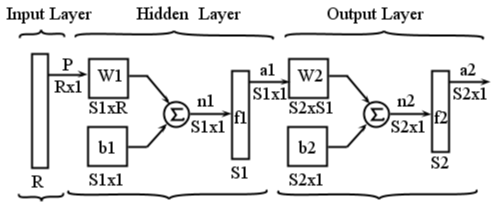
\includegraphics[width=350pt]{figures/MLP}
	\caption{Feedforward Multilayer Perceptron}
	\label{figure_mlp}
	\end{figure}
	
	
	% $$ n^{k+1}(i)=\sum\limits_{i=1}^{Sk}w^{k+1}(i,j)a^{k}(j)+b^{k+1}(i). $$
	\begin{equation}
	n^{k+1}_i=\sum\limits_{i=1}^{Sk}w^{k+1}_{ij}a^{k}_{j}+b^{k+1}_i
	\end{equation}\label{equation_feed_forward_input_to_k_layer}
	
	where $Sk$ is the number of neurons in the $k^{th}$ layer, $w^{k+1}_{ij}$ is the weight from $j^{th}$ neuron of layer $k$ to neuron $i$ of the layer $k+1$, $a^{k}_{j}$ is the output of neuron $j$ from the layer $k$ and $b^{k+1}_{i}$ is the bias connected to $i^{th}$ neuron in the layer $k+1$.
	
	The output of unit $I$ will be,
	%$$ a^{k+1}(i)=f^{k+1}(n^{k+1}(i))  $$
	\begin{equation}
	a^{k+1}_{i}=f^{k+1}(n^{k+1}_{i})
	\end{equation}\label{equation_feed_forward_output_from_k_layer}
	
	where $f^{k+1}(\cdot)$ is the activation function used in layer $k+1$
	
	For a $M$ layer network the system equations in the matrix form are given by
	
	\begin{align}\label{equation_feed_forward_step_in_matrix}
	a^{0}&=p\\
	a^{k+1}&= f^{k+1}(W^{k+1}a^k+b^{k+1}), k=0,1,2,...,M-1
	\end{align}
	
	Where $p$ is the input layer of the network
	
	The network learns association between a given set of input-output pairs ${(p_i,t_i), i=1,2,...,Q}$ for $Q$ number of training samples.
	
	
	%The performance index for the network is given as,
	%$$ V=\dfrac{1}{2}\sum\limits_{q=1}^{Q}(t_q-a^M_q)=\dfrac{1}{2}\sum\limits_{q=1}^{Q}e^T_q e_q $$
	%where $a^M_q$ is the output of the network when the $q^{th}$ input, $p_q$ is presented and $e_q=t_q-a^M_q$ is the error for the $q^{th}$ input.
	
	Now, next step of calculating feed forward quantities for all layers in the network is the back propagation training. In this phase we decide how neural network learn weights and biases with minimizing the generalization error. The quantity of weight and bias to adjust in the network parameters is send back to network from output layer to first hidden layer. In this research work Levenberg-Marquardt Backpropagation Learning rule is applied. Levenberg-Marquardt Backpropagation Learning algorithm is given in section \ref{lm_algorithm}.
	
	\paragraph{Levenberg-Marquardt (LM) Learning Algorithm \\\\}\label{lm_algorithm}
	
	
	 Many algorithms focus on standard numerical optimization, that is, using alternative methods for computing the weights associated with network connections. The most popular algorithms for this optimization are the conjugate gradient and Newton’s methods. Newton’s method is considered to be more efficient in the speed of convergence, but its storage and  computational requirements go up as the square of the size of the network.
	%  \cite{Hagan1994}. The LM algorithm is an approximation to Newton’s method [Moré77].
	The LM algorithm is efficient in terms of high speed of convergence and reduced memory requirements compared to the two previous methods. In general, with networks that contain up to several hundred weights, the LM algorithm has the fastest convergence \cite{Hagan1994}.
	
	For LM , the performance index to be minimized is defined as,
	\begin{equation}\label{lm_performance_index}
	F(w)=\sum\limits_{p=1}^{Q}{\sum\limits_{k=1}^{K}(t_{kp}-a_{kp})^2}
	\end{equation}
	
	where $w=[w_1 $ $ w_2 $ $ w_3 $ $ ...$ $  w_N]^T$ consists of all the weights of the network (including bias), $t_{kp}$ is the target value of the $k^{th}$ output and $p^{th}$ input pattern, $a_{kp}$ is the actual value of the $k^{th}$ output and $p^{th}$ input pattern, $N$ is the number of weights, and $K$ is the number of the network outputs.
	
	Equation (\ref{lm_performance_index}) can be written as
	\begin{equation}\label{equation_lm_error}
	F(w)=E^TE
	\end{equation}
	where
	$ E=[e_{11}$ $...$ $ e_{K1} $ $ e_{12}$ $...$ $ e_{K2}$ $ ...$ $ e_{1P} $ $...$ $ e_{KQ}]^T$
	
	$ e_{kp}=t_{kp}-a_{kp}, $ $ k=1,2,...,K, $ $ p=1,2,...,Q$
	where E is the cumulative error vector (for all input patterns).
	From equation (\ref{equation_lm_error}) the Jacobian matrix is defined as
	
	\begin{equation}\label{jacobian_matrix}
	 J=
	\begin{bmatrix}
	\frac{\partial{e_{11}}}{\partial{w_{1}}} & \frac{\partial{e_{11}}}{\partial{w_{2}}} & ... & \frac{\partial{e_{11}}}{\partial{w_{N}}} \\
	
	\frac{\partial{e_{21}}}{\partial{w_{1}}} & \frac{\partial{e_{21}}}{\partial{w_{2}}} & ... & \frac{\partial{e_{21}}}{\partial{w_{N}}} \\
	
	...&...&...&...&\\
	
	\frac{\partial{e_{K1}}}{\partial{w_{1}}} & \frac{\partial{e_{K1}}}{\partial{w_{2}}} & ... & \frac{\partial{e_{K1}}}{\partial{w_{N}}} \\
	
	...&...&...&...&\\
	
	\frac{\partial{e_{1Q}}}{\partial{w_{1}}} & \frac{\partial{e_{1Q}}}{\partial{w_{2}}} & ... & \frac{\partial{e_{1Q}}}{\partial{w_{N}}} \\
	
	\frac{\partial{e_{2Q}}}{\partial{w_{1}}} & \frac{\partial{e_{2Q}}}{\partial{w_{2}}} & ... & \frac{\partial{e_{2Q}}}{\partial{w_{N}}} \\
	...&...&...&...&\\
	
	\frac{\partial{e_{KQ}}}{\partial{w_{1}}} & \frac{\partial{e_{KQ}}}{\partial{w_{2}}} & ... & \frac{\partial{e_{KQ}}}{\partial{w_{N}}} \\
	\end{bmatrix}
	\end{equation}
	
	The increment of weights $\Delta{w}$ at iteration $t$ can be obtained as follows:
	\begin{equation}\label{equation_delta_w}
	%\Delta{w}=(J^T_tJ_t+\mu_tI)^{-1}J^T_tE_t
	\Delta{w}=-(J^TJ+\mu I)^{-1}J^TE
	\end{equation}
	where $I$ is identity matrix, $\mu$ is a learning parameter and $J$ is Jacobian of $K$ output errors with respect to $N$ weights of the neural network.
	
	Now the weights are calculated using the following equation
	\begin{equation}\label{equation_new_weight}
	w_{t+1}=w_t+\Delta{w}
	\end{equation}
	
	
	 For $\mu=0$ it becomes the Gauss-Newton method. For very large value of $\mu$ the LM algorithm becomes the steepest decent algorithm. The learning parameter $\mu$  is automatically adjusted at each iteration to meet the convergence criteria. The LM algorithm requires computation of the Jacobian matrix $J$ at each iteration and inverse of $J^TJ$ matrix of dimension $N$x$N$, This large dimensionality of LM algorithm is sometimes unpleasant to large size neural network.
	
	The learning parameter $\mu$ is updated in each iteration as follows. Whenever the $F(w)$ value is decreases, $\mu$ is multiplied by decay rate $\beta_{inc}$ whenever $F(w)$ is increases, $\mu$ is divided by decay rate $\beta_{dec}$ in new step.
	
	The LM Back-propagation training is illustrated in the Algorithm \ref{algorithm_lm}.
	
	\begin{algorithm}
	\caption{Levenberg-Marquardt Back-propagation Algorithm}
	\label{algorithm_lm}
	\begin{algorithmic}[1]
	\STATE Initialize the weights using Nguyen-Widrow weight initialization algorithm and parameter $\mu$.
	\STATE Compute the sum of the squared errors over all inputs $F(w)$.
	\STATE Solve Eq.(\ref{equation_delta_w}) to obtain the increment of weights.
	\STATE Recompute the sum of squared errors $F(w)$ using $w+\Delta{w}$ as trial w,and adjust
	\IF { trial $F(w)$ $\leq$ $F(w)$ in Step 2}
	\STATE $w=w+\Delta{w}$
	\STATE $\mu=\mu.\beta_{inc}$
	\STATE Goto Step 2.
	\ELSE
	\STATE $\mu=\frac{\mu}{\beta_{dec}}$
	\STATE  Goto Step 4.
	\ENDIF
	\end{algorithmic}
	\end{algorithm}
	
	\newpage
	\subsubsection{Radial Basis Function Network}
	\label{radial_basis_function}
	
	Radial-basis function network is used to perform a complex pattern classification task, the problem basically solved by transforming it into a high dimensional space in a non-linear manner. Non linear separability of complex patterns is justified by Cover's theorem,which stated as, ''A complex pattern-classification problem cast in a high dimensional space non-linearly is more likely to be linearly separable than in a low-dimensional space''.
	
	Radial basis functions are embedded into a two layer feed-forward network. Such a  network is characterized by a set of inputs and set of outputs. In between the inputs and outputs there is a layer of processing units called hidden units. Each of them implements a radial basis function. Generally there is a single hidden layer. In pattern classification problem inputs represent feature values, while each output corresponds to a class. A general RBF Network architecture is given in Figure \ref{figure_rbf}.
	
	\begin{figure}[hbtp]
	\centering
	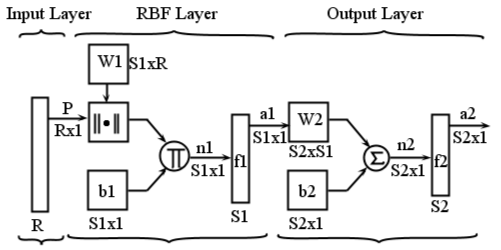
\includegraphics[width=350pt,height=170pt]{figures/RBF}
	\caption{RBF Neural Network}
	\label{figure_rbf}
	\end{figure}
	Let the input vector $x=[x_1,x_2,...,x_R]^T$ is feed to RBF Network.The network output can be obtained by
	
	\begin{equation}\label{equation_rbf_network_output}
	%t_k=\sum\limits_{j=1}^{M}w_{kj}\phi_j(\lVert x-c_j\rVert)+b_k
	t_k=\sum\limits_{j=1}^{M}w_{kj}\phi_j(x)+b_k
	\end{equation}
	where $\phi_j(\cdot)$ denotes the radial basis function of the $j^{th}$ hidden neuron, $w_{kj}$ denotes the hidden-to-output weight from $j^{th}$ hidden neuron to $k^{th}$ output neuron, $b_k$ denotes the bias connected to $k^{th}$ output neuron, and $M$ denotes the total hidden neurons.
	
	A radial basis function is a multidimensional function that describes the distance between a given input vector and a pre-defined centre vector. There are different types of radial basis function.  A normalized Gaussian function usually used as a radial basis function, which is given as
	
	\begin{equation}\label{equation_radial_basis_fuction}
	\phi_j(x)=\exp(-\frac{\Vert x-\mu_j\Vert^2}{2\sigma^2_j})
	\end{equation}
	where $\mu_j$ and $\sigma_j$ denote the centre and spread width of the $j^{th}$ neuron,respectively.
	
	Generally, the RBFNN training can be divided into two stages:
	\begin{enumerate}
	\item Determine the parameters of radial basis functions, i.e., Gaussian centre and spread width.
	\item Determine the output weight $w$ with supervised learning method. Usually Least-Mean-Square (LMS)
	\end{enumerate}
	The first stage is very crucial, since the number location of centres in the hidden layer will influence the performance of the RBFNN directly. In the next section, the principle and procedure of self-structure RBF algorithm will be described.
	
	\paragraph{Orthogonal Least Square Training Algorithm\\\\}\label{ols}
	
	Orthogonal Least Squares (OLS) is the most widely used supervised algorithm for radial basis neural network training. OLS is a forward stepwise regression procedure. Starting from a large pool of candidate centres ,i.e., from training examples, OLS sequentially selects the centre that results in the largest reduction of sum-square-error at the output.
	
	For $M$ basis vectors $\Phi=(\phi_1,\phi_2,...,\phi_M)$, orthogonal set $Q=(q_1,q_2,...,q_M)$ can be derived with the help of Grahm-Schmidt orthogonalization procedure as follows:
	
	\begin{align}
	q_1&=\phi_1 \label{q1} \\
	\alpha_{ik}&=\frac{q^T_i\phi_k}{q^T_iq_i} \; 1\le i \le k \label{alpha_ik}\\
	q_k&=\phi_k-\sum\limits_{i=1}^{k-1}\alpha_{ik}q_i \label{qk}\\
	& for \; k=2,3,...,M \nonumber
	\end{align}
	
	The orthogonal set of basis vectors Q is linearly related to the original set $\Phi$ by the relationship \cite{Chen1991} $ \Phi=QA \label{orthogonal_representation}$, where A is upper triangular matrix given by
	
	\begin{equation}
	A=
	\begin{bmatrix}
	1&\alpha_{12}&...&\alpha_{1M}\\
	0&1&&...\\
	...&&&\alpha_{M-1,M}\\
	0&...&0&1
	\end{bmatrix}
	\end{equation}
	
	Using this orthogonal representation, the RBF solution is expressed as
	\begin{equation}
	T=\Phi W= QG
	\end{equation}
	and the Least Square (LS) solution for the weight vector $G$ in the orthogonal space is
	
	\begin{equation}
	G=(Q^TQ)^{-1}Q^TT
	\end{equation}
	
	Since Q is orthogonal, $Q^TQ$ is then diagonal and each component of G can be extracted independently without ever having to compute a pseudo-inverse matrix,as
	
	\begin{equation}\label{ols_pseudo_inverse}
	g_i=\frac{q^T_iT}{q^T_iq_i}
	\end{equation}
	
	The sum of squares of the target vector T is given as
	
	\begin{equation}
	T^TT=\sum\limits_{i=1}^{M}g^2_iq^T_iq_i+E^TE
	\end{equation}
	
	OLS select a subset of regressors in stepwise forward manner by selecting the regressor $q_i$,which contributes to reduction of the error (relative to the total $T^TT$) by
	\begin{equation}\label{ols_error}
	[err]_i=\frac{g^2_iq^T_iq_i}{T^TT}
	\end{equation}
	
	The summary of Orthogonal Least Square RBF training \cite{Chen1991} is given in Algorithm \ref{algorithm_ols}.
	
	\begin{algorithm}
	\caption{OLS Algorithm}
	\label{algorithm_ols}
	\begin{algorithmic}[1]
	\STATE At the first step,for $1\le i\le M$, compute
	\STATE \qquad\qquad Orthogonalize vector: $q^{(i)}_1=\phi_i$
	\STATE \qquad\qquad Compute LS Solution:	$g^{(i)}_1=\frac{q^{{(i)}^T}_1T}{q^{{(i)}^T}_1q^{(i)}_1}$
	\STATE \qquad\qquad Compute error reduction: $[err]^{(1)}_i=\frac{g^{{(i)}^2}_1q^{{(i)}^T}_1q^{(i)}_1}{T^TT}$
	\STATE \quad select regressor that yields heights reduction in error $q_1=\arg_{q^{(i)}_1}\max[err]^{(i)}_1=\phi_{i_1}$
	
	
	\STATE At the $k^{th}$ step,for $1\le i\le M$, and $i$ not already selected
	\STATE \qquad\qquad Orthogonalize vector: $\alpha^{(i)}_{jk}=\frac{q^T_j\phi_i}{q^T_jq_j} \;, q^{(i)}_k=\phi_i-\sum\limits_{i=1}^{k-1}\alpha^{(i)}_{jk}q_j \;, for 1\le j \le k $
	\STATE \qquad\qquad Compute LS Solution:	$g^{(i)}_k=\frac{q^{{(i)}^T}_kT}{q^{{(i)}^T}_kq^{(i)}_k}$
	\STATE \qquad\qquad Compute error reduction: $[err]^{(1)}_k=\frac{g^{{(i)}^2}_kq^{{(i)}^T}_kq^{(i)}_k}{T^TT}$
	\STATE \quad select regressor $q_k=\arg_{q^{(i)}_k}\max[err]^{(i)}_k=\phi_{i_k}-\sum\limits_{j=1}^{k-1}\alpha_{jk}q_j$
	
	\STATE Stop at iteration M if rasidual error falls below pre-specified threshold $\epsilon$
	\STATE \qquad\qquad\qquad $1- \sum\limits_{j=1}^{M}[err]_j \le \epsilon $
	\STATE The regressors $\lbrace{\phi_{i_1},\phi_{i_2},\cdots,\phi_{i_M}}\rbrace$ define the final subset of RBF centers.
	\end{algorithmic}
	\end{algorithm}
	
	\section{Database Creation} \label{database_creation}
	
	To do experimentation with this research work, benchmark database for Off-line Nepali Handwritten Characters will be created. There will be three separate databases for Nepali handwritten consonants, vowels and numerals. More detail about Nepali consonant, vowel, and numeral database is given in the section \ref{section_consonant_database}, section \ref{section_vowel_database} and section \ref{section_numeral_database} respectively. Training and testing samples for recognition system will be then selected from each database in certain ratio.
	
	\subsection{Nepali Handwritten Consonant Database}
	\label{section_consonant_database}
	
	Nepali language contains $36$ Devanagari alphabets for Consonants. Figure \ref{figure_ka_kha} shows one sample for Nepali handwritten consonants. To create training and testing database for recognition system, handwritten consonant images are scanned with digital scanner and cropped for individual characters. There will be about $1000$ samples for each $36$ classes of consonants. Samples will be taken from different writers.
	\begin{figure}[hbtp]
	\centering
	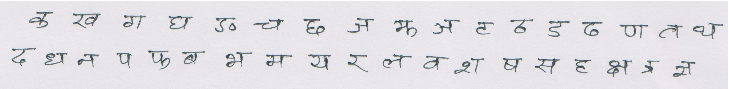
\includegraphics[width=\linewidth]{figures/ka_kha}
	\caption{Nepali Handwritten Consonants}
	\label{figure_ka_kha}
	\end{figure}
	
	\subsection{Nepali Handwritten Vowel Database}
	\label{section_vowel_database}
	Nepali language contains $12$ Devanagari alphabets for vowels. Figure \ref{figure_a_aa} shows one sample for Nepali handwritten vowels. To create training and testing database for recognition system, handwritten vowel samples are scanned with digital scanner and cropped for individual characters. There will be about $1000$ samples for each $12$ classes of vowels. Samples will be taken from different writers.
	\begin{figure}[hbtp]
	\centering
	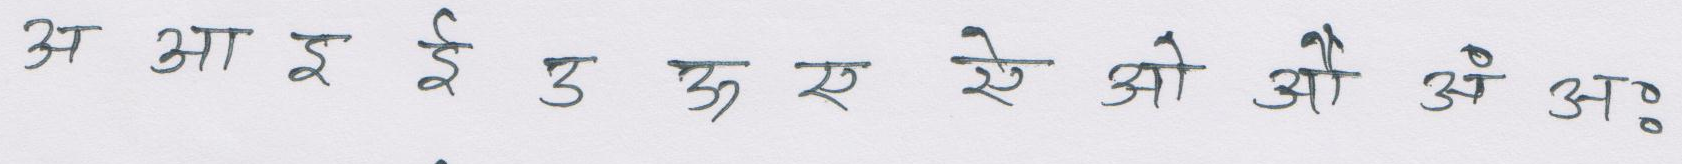
\includegraphics[width=\linewidth]{figures/a_aa}
	\caption{Nepali Handwritten Vowels}
	\label{figure_a_aa}
	\end{figure}
	
	\subsection{Nepali Handwritten Numeral Database}
	\label{section_numeral_database}
	
	Nepali language contains $10$ Devanagari numerals. Figure \ref{figure_one_two} shows one sample for Nepali handwritten numerals. To create training and testing database for recognition system, handwritten numeral images are scanned with digital scanner and cropped for individual characters. There will be about $1000$ samples for each $10$ classes of numerals. Samples will be taken from different writers.
	\begin{figure}[hbtp]
	\centering
	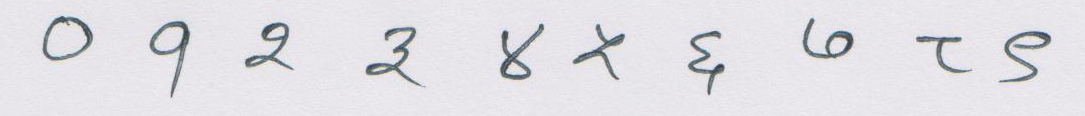
\includegraphics[width=\linewidth]{figures/one_two}
	\caption{Nepali Handwritten Numerals}
	\label{figure_one_two}
	\end{figure}
	
	\section{Expected Result}\label{expected_result}
	
	The attainable accuracy and efficiency defined by the Recognition models could be achieved as a final result.
	\section{Working Schedule}\label{working_schedule}
	Working Schedule for the dissertation work is given below. Horizontal axis contain the time slots for the work. Each slot represent one week  of time. Vertical axis contain tasks to be done.\par
	
		\centering
		\scalebox{0.9}{
			\begin{ganttchart}[x unit=0.80 cm, 
				y unit title=0.7cm,
				y unit chart=0.5cm, vgrid, title label font=\footnotesize,
				canvas/.style={draw=black, dotted}]{1}{16}
				\gantttitle{Weeks}{16}\\
				\gantttitlelist{1,2,3,4,5,6,7,8,9,10,11,12,13,14,15,16}{1} \\
				
				\ganttbar{Study and Analysis}{1}{4}     \\ 
				\ganttbar{Proposal Writing}{4}{5}     \\ 
				\ganttmilestone{Proposal Presentation}{5}     \\ 
				\ganttbar{Data Collection}{5}{8}    \\   
				\ganttbar{Implementation}{5}{10}              \\ 
				\ganttbar{Testing} {8}{10} \\
				\ganttbar{Final Documentation} {6}{14} \\
				\ganttbar{Review} {14}{15} \\
				\ganttmilestone {Final Presentation} {16}
			\end{ganttchart}}
			
	\bibliographystyle{ieeetr}
	%\include{References}
	\bibliography{references}
	\end{document}
	
	% Dedication
	%\newpage
	%\begin{center}
	%\vspace*{2in}
	%{\it for Randy and Charles}
	%\end{center} 